\documentclass[a4paper,10pt]{article}
\usepackage[applemac]{inputenc} %\usepackage[utf8]{inputenc}
\usepackage[pdftex]{graphicx}
\usepackage{url}

\title{Arduino Laser Actuator}
\author{InThe - Aclaro}
\date{2012-09-01}

\pdfinfo{%
  /Title    (Arduino L�ser Actuator)
  /Author   (Josep)
  /Creator  ()
  /Producer ()
  /Subject  ()
  /Keywords ()
}

\begin{document}
\maketitle

\section{Desenvolupament del prototip}
\subsection{Descripci�}
En aquest prototip s'implementar� un posicionador de l�ser a partir de la detecci� de moviment.


\begin{figure}[htbp] %  figure placement: here, top, bottom, or page
   \centering
	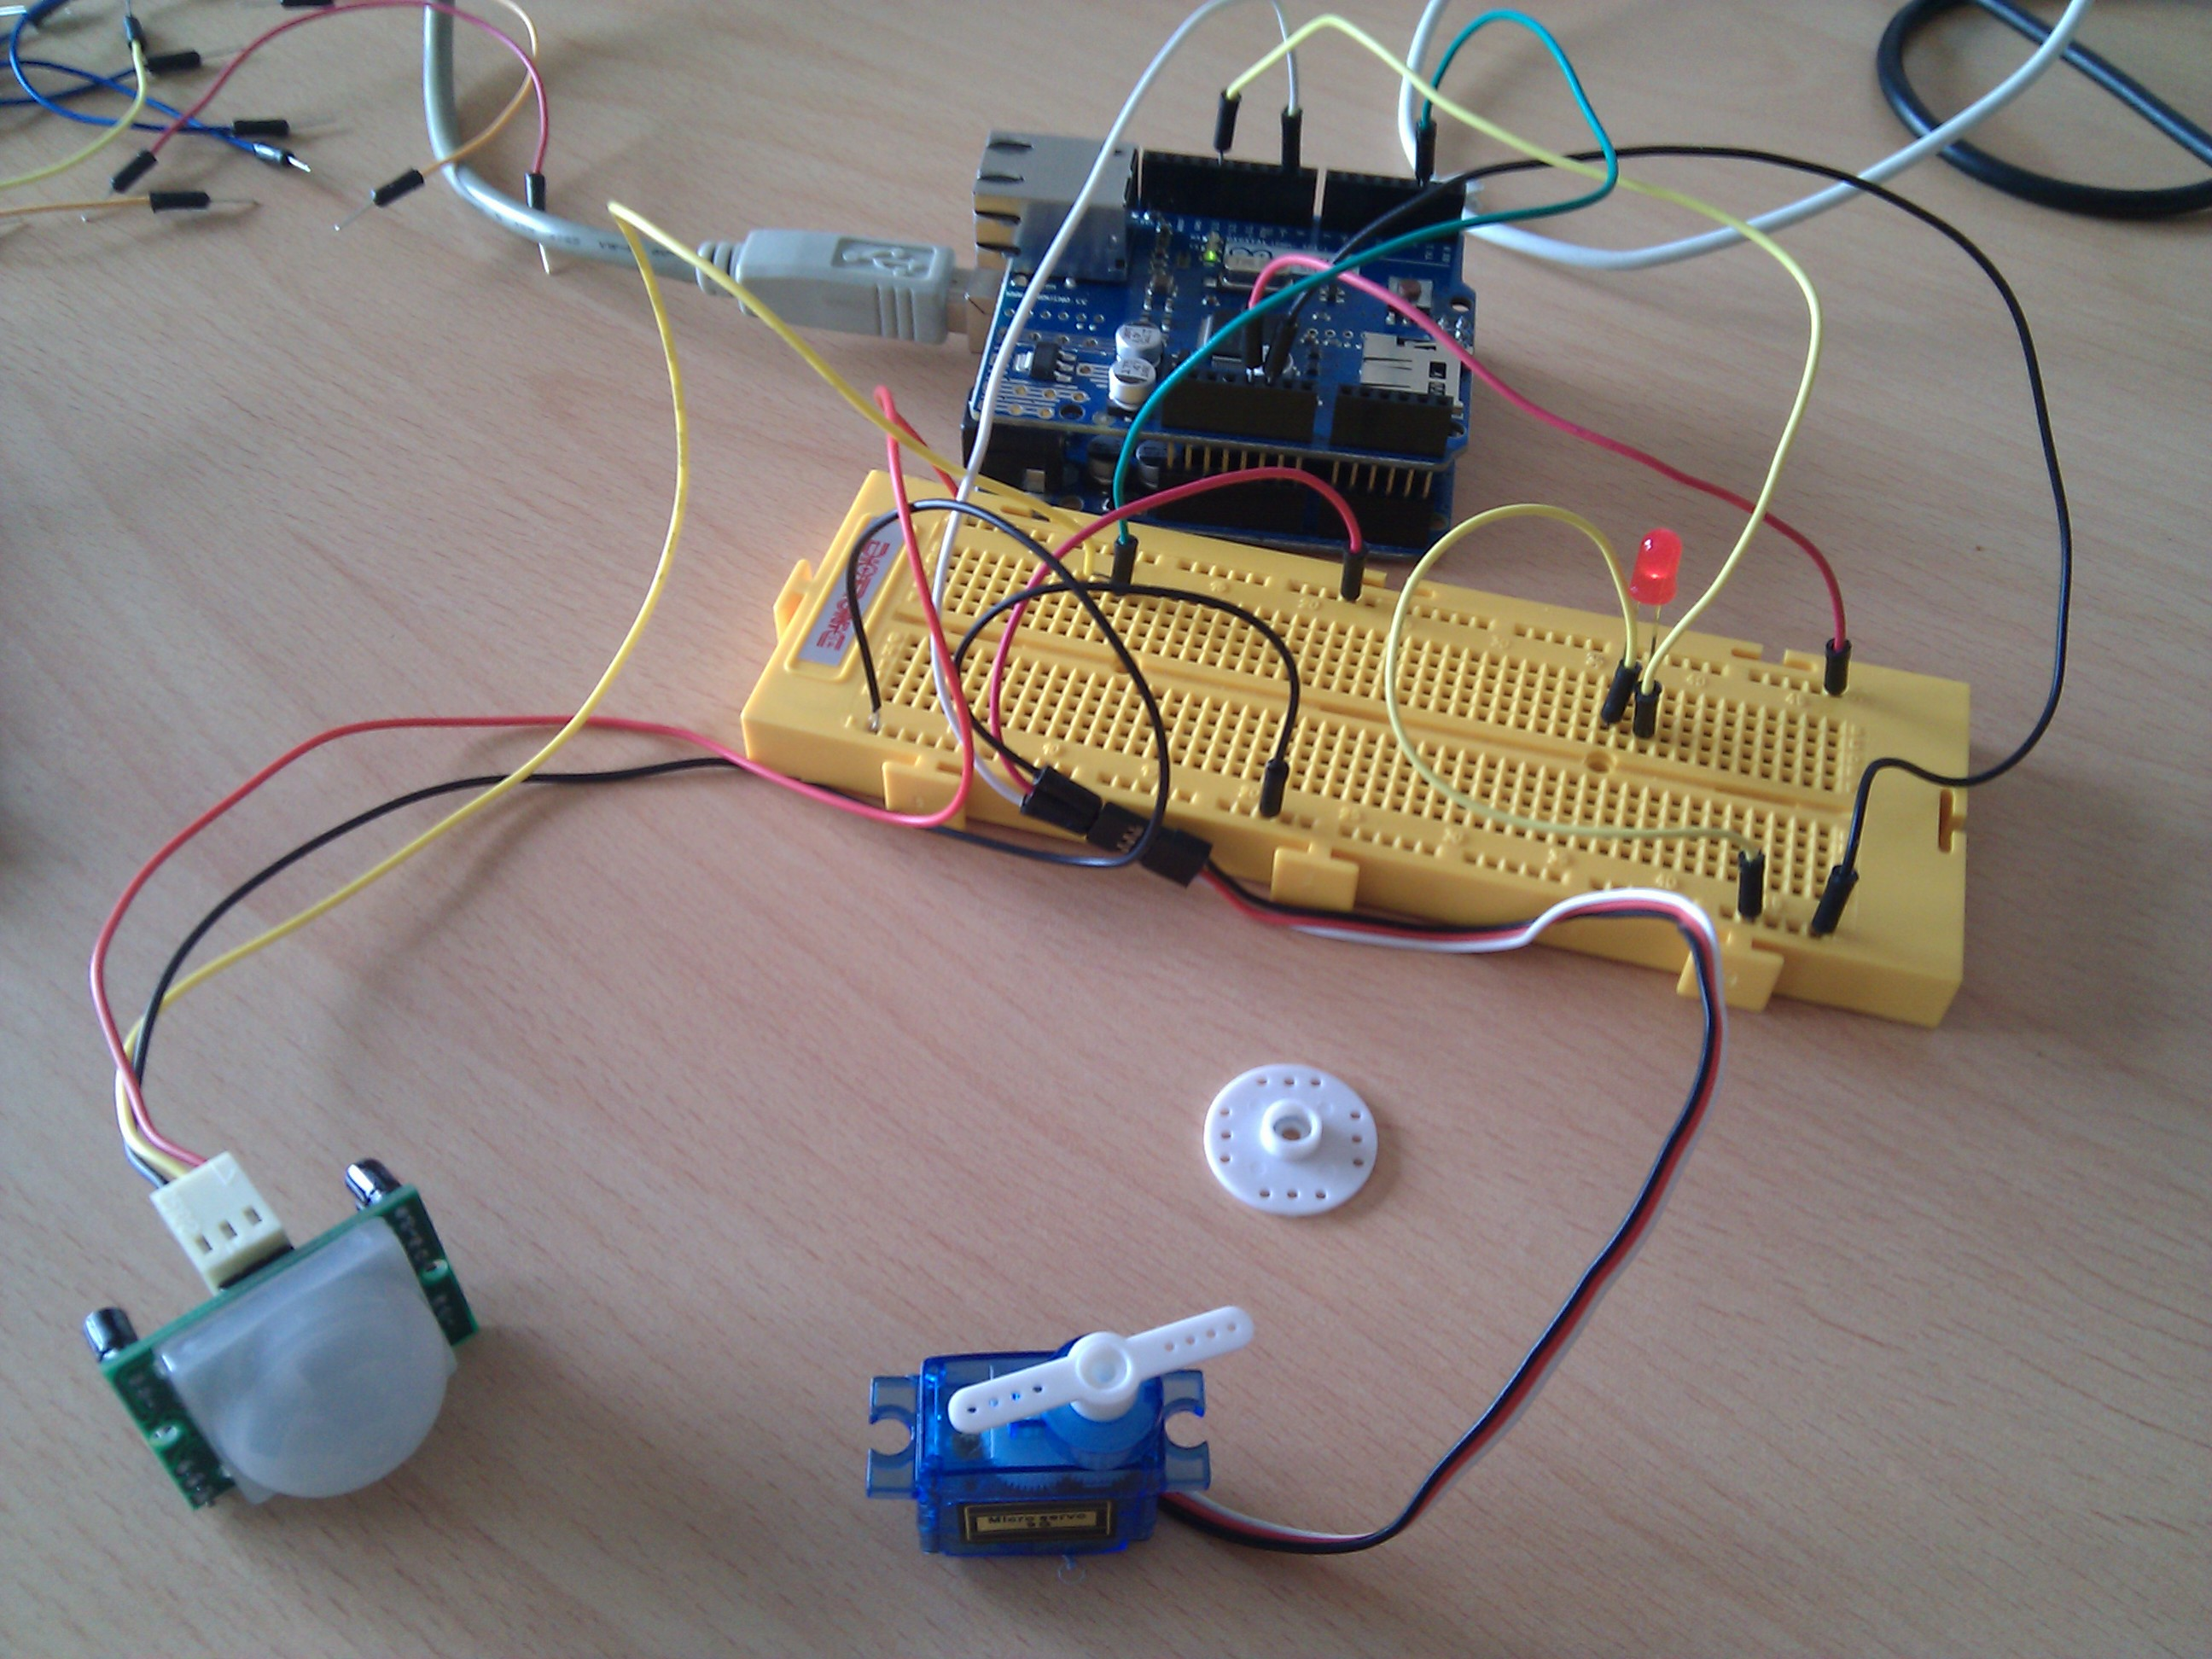
\includegraphics[width=1.0\textwidth]{images/muntatge} 
   \caption{Posicionador de l�ser amb detector de moviment}
   \label{fig:example}
\end{figure}

\subsection{Material}
\begin{itemize}
	\item Arduino Uni
	\item Protoboard
	\item cables
	\item PIR sensor
	\item Servo motor
\end{itemize}


\pagebreak
\subsection{Codi}

\scriptsize
\begin{verbatim}
/* 
 laser_actuator 
 Creat:     2012-08-29 (Josep)
 Modificat: 2012-09-01 (Josep)
*/

#include <Servo.h>

int led = 13;
int motionPin = 2;
int actuatorPin = 9;

Servo actuator;

void setup() {
  pinMode(led, OUTPUT);
  pinMode(motionPin, INPUT);
  actuator.attach(actuatorPin);
}
void loop() {
  int motionVal = digitalRead(motionPin);
  if (motionVal == HIGH) {
    digitalWrite(led, HIGH);
    espanta();
  }else{
    digitalWrite(led, LOW);
  }
}


/*
  Funcio espanta()
  Posa el laser a 0�, 90�, 18�0 i torna a 0� en intervals d' 1 segon
*/
void espanta(){
  actuator.write(0);
  delay(1000);
  actuator.write(90);
  delay(1000);
  actuator.write(180);
  delay(1000);
  actuator.write(0);
}
\end{verbatim}
\normalsize

En el moment que el sensor PIR detecta moviment es posiciona el motor a 0�, passat un segon a 90�, passat un altre segon a 180� i un segon m�s tard a la posici� inicial de 0�.

Aquest proc�s es repeteix fins que el sensor no detecti m�s moviment. Hem de tenir en compte que aquest sensor no detecta pres�ncia, nom�s moviment.

\pagebreak
\begin{thebibliography}{9}

\bibitem{arduino-web}  P�gina web d'Arduino: 
  
	\url{http://arduino.cc/}

\bibitem{github-project} Projecte a GitHub

	\url https://github.com/apuratepp/ArduinoLaserActuator

\end{thebibliography}

\end{document}
